---
id: tkz-euclide-ejemplo-36
title: "Sectores Poligonales"
description: "Dibuja y colorea varios sectores circulares consecutivos de un mismo radio."
keywords: [sectores, circulares, radio, relleno, colores]
tags: [tkzDrawSector, tkzFillSector]
sort: 36
---
\documentclass[tikz,border=2mm]{standalone}
\usepackage{tkz-euclide}

\begin{document}
    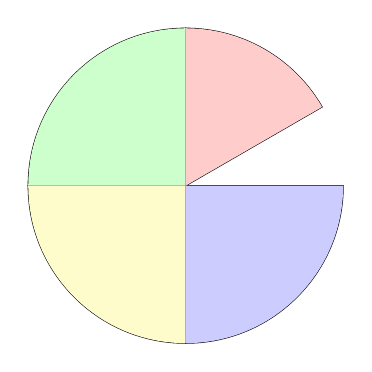
\begin{tikzpicture}
        % Define el centro O del círculo y un punto auxiliar A (opcional).
        \tkzDefPoint(0,0){O}
        \tkzDefPoint[shift={(0,0)}](30:2){A}
    
        % Dibuja cuatro sectores circulares (cuadrantes) de radio 2.
        \tkzDrawSector[R](O,2)(30,90)
        \tkzDrawSector[R](O,2)(90,180)
        \tkzDrawSector[R](O,2)(180,270)
        \tkzDrawSector[R](O,2)(270,360)
    
        % Rellena cada sector con un color distinto.
        \tkzFillSector[R,fill=red!20](O,2)(30,90)
        \tkzFillSector[R,fill=green!20](O,2)(90,180)
        \tkzFillSector[R,fill=yellow!20](O,2)(180,270)
        \tkzFillSector[R,fill=blue!20](O,2)(270,360)
    \end{tikzpicture}
\end{document}
